\Chapter{ARTICLE 2 : MODELLING RESISTANCE WELDING OF THERMOPLASTIC COMPOSITES WITH A NANOCOMPOSITE HEATING ELEMENT}\label{sec:Theme2}

\selectlanguage{french}
\section{Introduction}

Cet article présente les travaux de modélisation du soudage résistif de composites thermopastiques avec un élément chauffant nanocomposite. Ces travaux avaient pour but d'optimiser les performances mécaniques des joints et établir une fenêtre d'opération. La planification des travaux, la réalisation des expériences, l'analyse des résultats et la rédaction de cet article ont été réalisés par David Brassard. Martine Dubé et Jason R. Tavares ont supervisés l'ensemble des travaux et ont contribués à la révision de l'article. 

\textbf{Auteurs} : David Brassard, Martine Dubé et Jason R. Tavares

\textbf{Article soumis dans la revue} : Composites Part B: Engineering

\textbf{Date de soumission} : 7 octobre 2019

\textbf{Mots clés} : Resistance welding; Finite element analysis (FEA); Thermoplastic resin; \\ Joints/joining

\selectlanguage{english}

\section{Abstract}

Electrically conductive nanocomposite heating elements are being developed as a complement to traditional carbon fibre or stainless steel heating elements in resistance welding of thermoplastic composites. 
Here we present the development of a finite element model of the resistance welding process with these new heating elements, from which we establish a process window for high quality welded joints. 
The finite element model results were validated experimentally and a lap shear strength improvement of 28\% is reported relative to previously published results. 
Fractography analysis of the broken joints revealed a thin-layer cohesive failure mode due to the brittleness of the nanocomposite heating elements. 

%%%%%%%%%%%%%%%%%%%%%%%%%%%%%%%%%%%%%%%%%%%%%%%%%%%%%%%%%%%%%%%%%
\section{Introduction}
%%%%%%%%%%%%%%%%%%%%%%%%%%%%%%%%%%%%%%%%%%%%%%%%%%%%%%%%%%%%%%%%%

The use of thermoplastic composite (TPC) materials is rising \cite{Mathijsen2016} and these materials now find applications in wind turbine and aerospace industries \cite{Penumadu2019}. 
Their short processing cycle, improved impact resistance, end-of-life recyclability and chemical stability \cite{cogswell1992} make them good candidates for lightweight structural components compared to traditional thermoset resins. 
A major difference between thermosets and thermoplastics is the methods to join parts together: while adhesive bonding and mechanical assembly is the norm for thermoset composites, assemblies of TPCs are preferably produced by welding together individual components. 
This is achieved by localized heating of the weld zone through resistance, induction or ultrasonic welding. 
During resistance welding, the weld zone temperature increases via joule heating of a resistive heating element (HE) located between the adherents \cite{Ageorges2001a,Stavrov2005a,Dube2007c,Shi2014,Brassard2019a,Eveno1988} (Fig. \ref{fig:2_Fig1}). 
This process offers good mechanical performance and short processing times of the order of minutes, and can be achieved with HE such as carbon fibre plies \cite{Eveno1988}, stainless steel (SS) meshes \cite{Stavrov2005a,Dube2007c,Shi2014} or, more recently, an electrically conductive nanocomposite polymer \cite{Brassard2019a}. 

\begin{figure}[ht]
	\center
	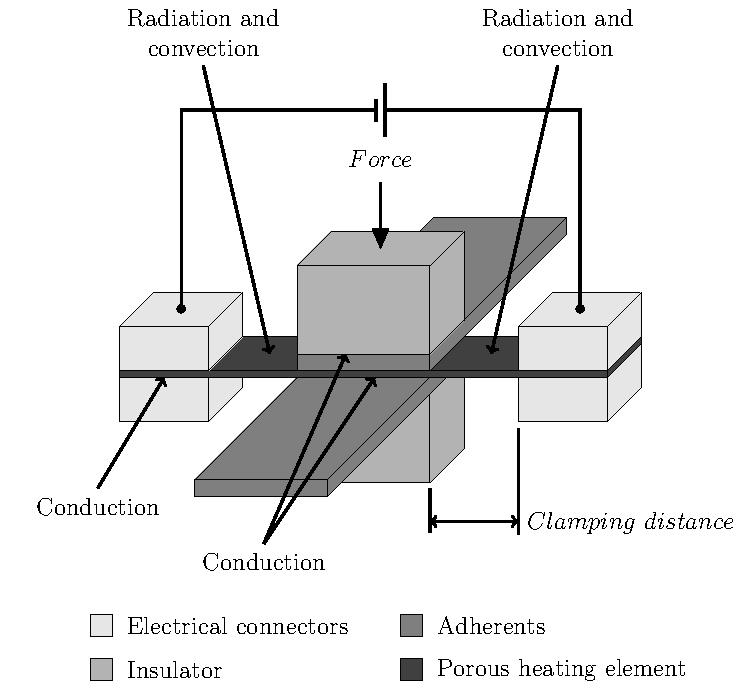
\includegraphics[scale=1]{2_Fig1}
	\caption{Schematic view of the resistance welding process highlighting local thermal transport mechanisms \cite{Brassard2019b}}
	\label{fig:2_Fig1}
\end{figure} 

It was recently shown that an electrically conductive nanocomposite polymer HE can successfully weld unidirectional (UD) carbon fibre reinforced PEEK (CF/PEEK) composite adherents \cite{Brassard2019a}. 
While this proof-of-concept illustrated how the new HE could complement SS meshes and carbon fibre HE, the effects of the welding parameters on the weld quality were not thoroughly explored. 
The development of a processing window is needed to assess the full capabilities of the nanocomposite HE. 

The main parameters controlling the resistance welding process are the power density (electrical power divided by the heating element area), duration, welding pressure, geometry of the components of the jig holding the adherents and the properties of the materials used as thermal insulators. 
Good control of the heating parameters is required to keep the heat-affected zone (HAZ) as close as possible to the bonding surfaces to avoid deconsolidation and fibre movements \cite{Stavrov2005a}. 
The power density and process duration affect the size and shape of the HAZ by controlling the rate and amount of energy dissipated within the weld, while pressure on the laminates prevents the formation of porosity from deconsolidation of the plies \cite{Shi2017}. 
For a given welding jig configuration, the clamping distance and the dimensions and nature of the electrodes dictate edge effects, which are caused by the sharp transition in the heat dissipation mechanism of the HE from conduction in the weld and adherents to radiation and potentially convection outside the weld as illustrated in Fig. \ref{fig:2_Fig1} \cite{Ageorges2001b}. 
Edge effects can have a strong impact on the temperature distribution within the weld. 
Inappropriate adjustment of the clamping distance may lead to incomplete welding or degradation at the edges \cite{Talbot2013}. 
Finally, the thermal properties and geometry of the insulators will have a strong impact on optimal processing parameters, making those parameters dependant on the design of the welding jig. 
Going from an experimental jig to a production setup requires careful considerations and a deep understanding of the welding process. 

A process window that compounds all these effects cannot be obtained solely through physical experiments, because key processing information is unavailable. 
Namely, the inability to install thermocouples within the weld without disturbing the process limits the ability to measure the temperature at the interface when using a nanocomposite HE. 
However, information gained through preliminary experiments can be used to help developing a finite element model of resistance welding with a nanocomposite HE, which will in turn guide subsequent exploration of the welding parameters. 

Therefore, this article presents the development and validation of a transient finite element model for resistance welding of thermoplastic composites with a nanocomposite HE. 
This model is subsequently used to predict good welding conditions and establish a processing window leading to improved mechanical performances. 

%%%%%%%%%%%%%%%%%%%%%%%%%%%%%%%%%%%%%%%%%%%%%%%%%%%%%%%%%%%%%%%%%
\section{Methodology}
%%%%%%%%%%%%%%%%%%%%%%%%%%%%%%%%%%%%%%%%%%%%%%%%%%%%%%%%%%%%%%%%%

%%%%%%%%%%%%%%%%%%%%%%%%%%%%%%%%%%%%%%%%%%%%%%%%%%%%%%%%%%%%%%
\subsection{Resistance welding finite element model}
%%%%%%%%%%%%%%%%%%%%%%%%%%%%%%%%%%%%%%%%%%%%%%%%%%%%%%%%%%%%%%

A transient finite element model of the resistance welding process is developed with the COMSOL Multiphysics\textregistered \ software. 
The model evaluates the effects of welding parameters on the temperature distribution and profile in the joint over time with the goal of establishing a processing window leading to good weld quality and mechanical performance based on these results. 
This model evaluates the electrical field in the electrodes and nanocomposite HE, joule heating of the nanocomposite HE, heat transfer in the solids, heat dissipation through convection and radiation and thermal contact conductance between critical components. 
The geometry of the components is detailed in Fig. \ref{fig:2_Fig2}. 
The gaps identified in the geometry were \mbox{0.1\,mm}.

\begin{figure}[h!]
	\center
	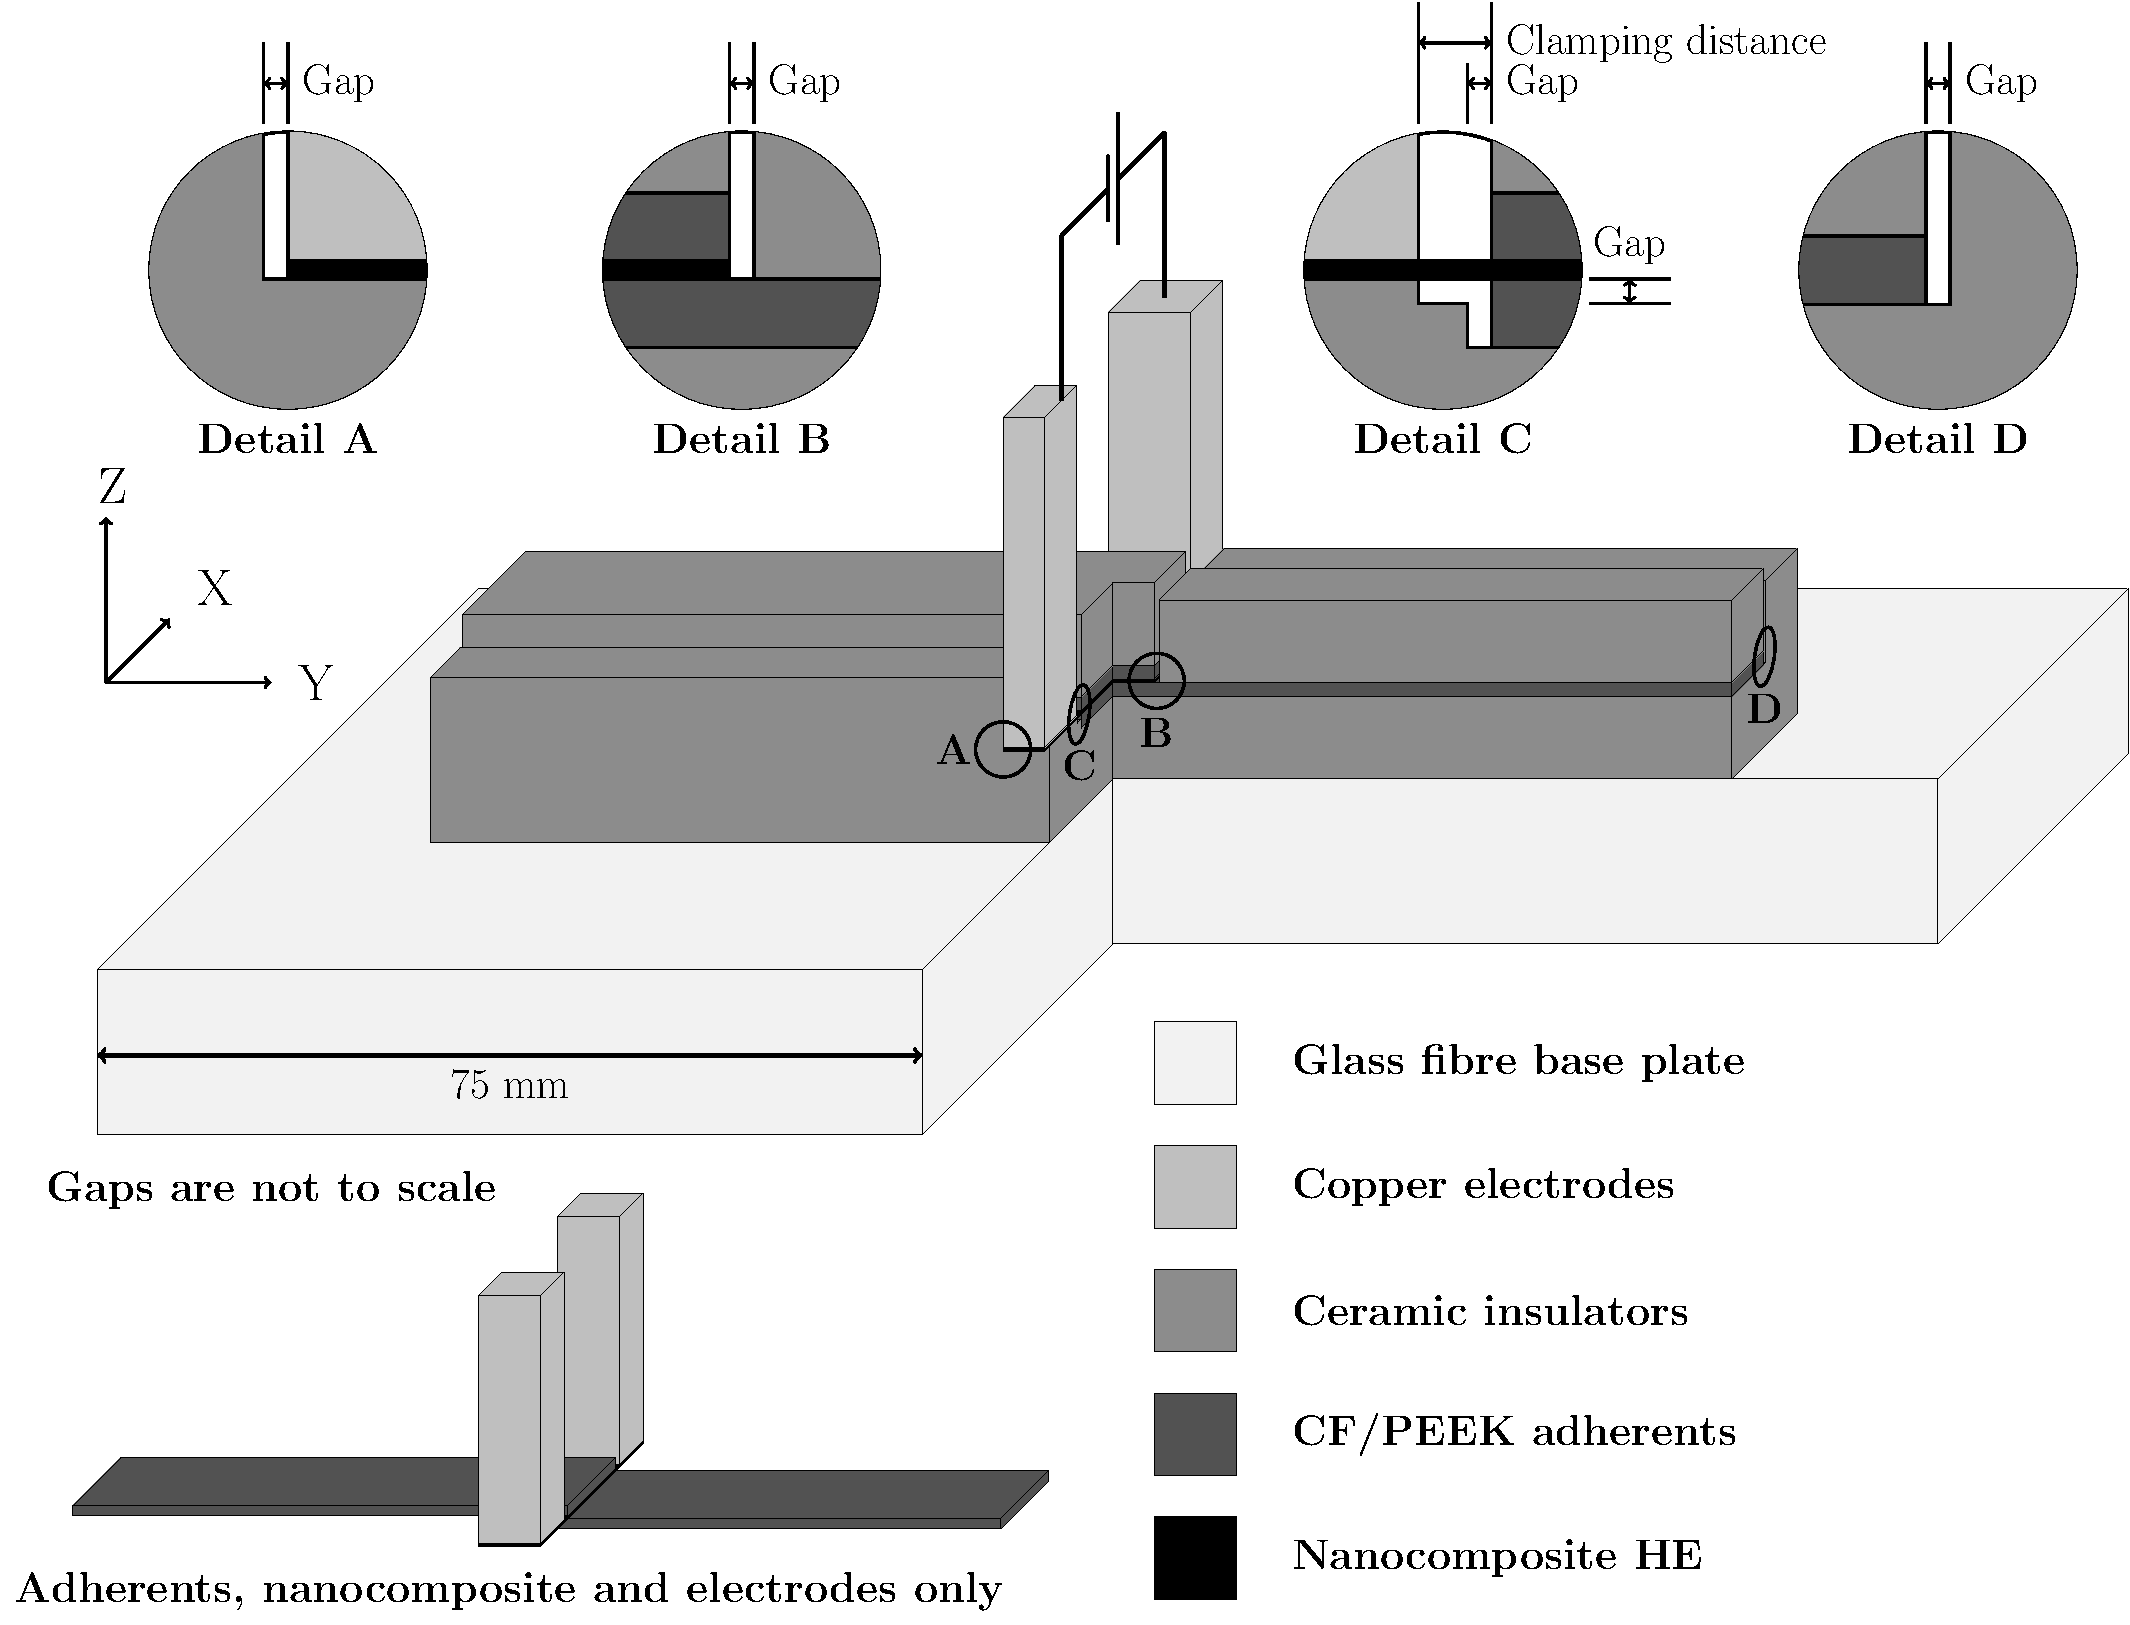
\includegraphics[width=0.9\textwidth]{2_Fig2}
	\caption{Three-quarter section view of the geometry of the model highlighting the components of the model and location of the 0.1 mm air gaps \cite{Brassard2019b}}
	\label{fig:2_Fig2}
\end{figure} 

\FloatBarrier
%%%%%%%%%%%%%%%%%%%%%%%%%%%%%%%%%%%%%%%%%%%%%%%%%%%%%%%%%%%%%%
\subsubsection{Electrical field evaluation}
%%%%%%%%%%%%%%%%%%%%%%%%%%%%%%%%%%%%%%%%%%%%%%%%%%%%%%%%%%%%%%

The model evaluates the electrical field in the nanocomposite HE and the electrodes. 
The resulting field is used to compute the joule losses from current and electrical resistance. 
The constitutive rules for conservation of current and charges are imposed, with the application of the general equations \ref{eq:current_conservation_1} to \ref{eq:current_conservation_3} describing the electrical field within the nanocomposite HE and the copper electrodes. 
The equation of continuity (Eq. \ref{eq:current_conservation_1}) defines that the divergence ($\nabla$) of the current density ($\mathbf{J}$) is equal to the current source ($Q_j$) (both expressed in \mbox{A\,m$^{-2}$}). 
Ohm’s law (Eq. \ref{eq:current_conservation_2}) defines that the current density ($\mathbf{J}$) is equal to the sum of imposed external current density ($\mathbf{J_e}$ in \mbox{A\,m$^{-2}$}) and the product of the sum of the electrical conductivity ($\sigma$ in \mbox{S\,m$^{-1}$}) and the product of the permittivity of vacuum ($\varepsilon_0$ in \mbox{F\,m$^{-1}$}) and the relative permittivity ($\varepsilon_r$ a dimensionless value) as function of time with the electric field ($\mathbf{E}$ in \mbox{V\,m$^{-1}$}). 
Finally, Eq. \ref{eq:current_conservation_3} defines the electric field ($\mathbf{E}$ in \mbox{V\,m$^{-1}$}) as the negative of divergence ($\nabla$) of the electric potential ($V$ in V). 

\begin{equation}
\nabla \cdot \mathbf{J} = Q_j
\label{eq:current_conservation_1}
\end{equation}

\begin{equation}
\mathbf{J} = \left( \sigma + \varepsilon_0 \varepsilon_r \frac{\partial}{\partial t} \right) \mathbf{E} + \mathbf{J_e}
\label{eq:current_conservation_2}
\end{equation}

\begin{equation}
\mathbf{E} = - \nabla V
\label{eq:current_conservation_3}
\end{equation}

As in the laboratory experiment, a constant power input was applied to the top surface of an electrode as boundary condition. 
The top surface of the second electrode was set as a ground connection with an electrical tension of 0\,V. 
The other outer edges of the nanocomposite and electrodes were considered as electrical insulators and their boundary conditions were defined as per equation \ref{electrical_insulation} which defines that the current density perpendicular to the boundary is equal to 0. 

\begin{equation}
\mathbf{n} \cdot \mathbf{J} = 0
\label{electrical_insulation}
\end{equation}

%%%%%%%%%%%%%%%%%%%%%%%%%%%%%%%%%%%%%%%%%%%%%%%%%%%%%%%%%%%%%%
\subsubsection{Heat transfer within solids}
%%%%%%%%%%%%%%%%%%%%%%%%%%%%%%%%%%%%%%%%%%%%%%%%%%%%%%%%%%%%%%

An energy balance (Eq. \ref{eq:thermal_balance}) with Fourier’s law of heat conduction is calculated for all constituents of the model. 

\begin{equation}
Q_e= \rho C_p \frac{\partial T}{\partial t} + \nabla \cdot -k \nabla T
\label{eq:thermal_balance}
\end{equation}

The one-way coupling between the thermal and electrical components of the model is obtained through an electromagnetic heat source from resistive losses ($Q_e$).  
That heat source is defined (Eq. \ref{electromagnetic_heat_source_term}) as the product of the current density ($\mathbf{J}$ in \mbox{A\,m$^{-2}$}) and the electric field ($\mathbf{E}$ in \mbox{V\,m$^{-1}$}). 

\begin{equation}
Q_e =  \mathbf{J} \cdot \mathbf{E} 
\label{electromagnetic_heat_source_term}
\end{equation}

The boundary layer thickness was evaluated with the Boussinesq approximation to confirm on which surfaces convective cooling boundary conditions should be considered. 
For $Pr > 0.6 $, the thickness can be evaluated with Eq. \ref{eq:boundary_layer_thickness} with the Grashof number for a specific length ($Gr_L$) defined as in Eq. \ref{eq:grashof_number}. 
To confirm the validity of this equation, the Prandtl number ($Pr$) was evaluated with Eq. \ref{eq:prandtl_number}. 
Based on the properties of air, the boundary layer thickness was evaluated to be at least \mbox{5\,mm} thick for a specific length of \mbox{12.7\,mm} that is representative of the height of the section enclosed between the sides of the welded joint and the electrodes. 

\begin{equation}
\delta = 5 L \left( \frac{Gr_L}{4} \right)^{-\sfrac{1}{4} }
\label{eq:boundary_layer_thickness}
\end{equation}

\begin{equation}
Gr_L = \frac{g \beta \left( T_s - T_{\infty} \right) L^3}{\nu^2}
\label{eq:grashof_number}
\end{equation}

\begin{equation}
Pr = \frac{C_p \mu}{k}
\label{eq:prandtl_number}
\end{equation}

Considering that the clamping distance (Fig. \ref{fig:2_Fig2}) is usually less than \mbox{2\,mm}, it is assumed that no convective cooling takes place in the gaps of the model and in the enclosed space between the sides of the composite and the electrodes. 
For the other outer surfaces of the model, natural convection described as in Eq. \ref{eq:natural_convection} is applied. 
The natural convection coefficient ($h_{conv}$) for vertical surfaces with $10^4 < Pr \ Gr < 10^9$ can be approximated with Eq. \ref{eq:convection_vertical_plate} at \mbox{20\,W\,m$^{-1}$\,K$^{-1}$}.
This value is applied as a constant in the model for all outer surfaces. 

\begin{equation}
-\mathbf{n} \cdot \mathbf{q} = -h_{conv} \left( T_s -T_{\infty} \right)
\label{eq:natural_convection}
\end{equation}

\begin{equation}
h = \frac{0.59 \lambda_{air} \left(Pr \ Gr_L\right)^{0.25}}{L_c}
\label{eq:convection_vertical_plate}
\end{equation}

The surface temperature of the exposed sections of the nanocomposite is high enough that radiative cooling must be accounted for, as defined in Eq. \ref{eq:radiative_cooling} with an emissivity of 1. 

\begin{equation}
- \mathbf{n} \cdot \mathbf{q} = \varepsilon \sigma_{SB} \left( T_{\infty}^4 - T_s^4 \right) 
\label{eq:radiative_cooling}
\end{equation}

The surfaces within the gaps of the model are considered to be thermally isolated to simulate imperfect contact between the insulator blocks.

%%%%%%%%%%%%%%%%%%%%%%%%%%%%%%%%%%%%%%%%%%%%%%%%%%%%%%%%%%%%%%
\subsubsection{Thermal contact conductance}
%%%%%%%%%%%%%%%%%%%%%%%%%%%%%%%%%%%%%%%%%%%%%%%%%%%%%%%%%%%%%%

Imperfect thermal contact between components is simulated with a thermal contact resistance that is inserted between the composite adherents and the ceramic insulators in the sections directly above and under the welded zone. 
The Cooper-Mikic-Yovanivich correlation \cite{Cooper1969} (Eq. \ref{eq:conductance_coefficient} to \ref{eq:asperities_slope}) which is based on the surfaces roughness, the contact pressure and physical properties defines a thermal contact conductance coefficient ($h_c$). 
For the conductance of the interstitial gas ($h_g$), a value of \mbox{0.0262\,W\,m$^{-2}$\,K$^{-1}$} was used to simulate air \cite{rumble2019crc}. 
The total conductance coefficient ($h$) is then applied in the model as shown in Eq. \ref{eq:contact_conductance_surface1} and \ref{eq:contact_conductance_surface2}. 

\begin{equation}
h = h_c + h_g
\label{eq:conductance_coefficient}
\end{equation}

\begin{equation}
h_c = 1.25 \times k_{contact} \frac{m_{asp}}{\sigma_{asp}} \left( \frac{p}{H_c} \right)^{0.95}
\label{eq:cmy_correlation}
\end{equation}

\begin{equation}
\frac{1}{k_{contact}} = \frac{1}{2} \left( \frac{1}{k_1} + \frac{1}{k_2} \right)
\label{eq:contact_conductivity}
\end{equation}

\begin{equation}
\sigma_{asp} = \sqrt{\sigma_{asp,1}^2 + \sigma_{asp,2}^2}
\label{eq:asperities_average_height}
\end{equation}

\begin{equation}
m_{asp} = \sqrt{m_1^2 + m_2^2}
\label{eq:asperities_slope}
\end{equation}

\begin{equation}
-\mathbf{n_1} \cdot \left( -k_1 \nabla T_1 \right) = -h \left( T_2 -T_1 \right)
\label{eq:contact_conductance_surface1}
\end{equation}

\begin{equation}
-\mathbf{n_2} \cdot \left( -k_2 \nabla T_2 \right) = -h \left( T_1 -T_2 \right)
\label{eq:contact_conductance_surface2}
\end{equation}

%%%%%%%%%%%%%%%%%%%%%%%%%%%%%%%%%%%%%%%%%%%%%%%%%%%%%%%%%%%%%%
\subsection{Material}
%%%%%%%%%%%%%%%%%%%%%%%%%%%%%%%%%%%%%%%%%%%%%%%%%%%%%%%%%%%%%%

The matrix of the nanocomposite HE is composed of polyetherimide (PEI) (CAS 61128-46-9) pellets ordered from Sigma Aldrich. 
It has a melt index of 18\,g per 10\,min at 337\,$^{\circ}$C with a mass of 6.6\,kg and its molecular weight is $M_n$ of \mbox{15.0\,kg\,mol$^{-1}$} and $M_w$ of \mbox{21.6\,kg\,mol$^{-1}$}. 
To obtain a conductive nanocomposite, dry powdered \mbox{MWCNTs}, produced by combustion chemical vapour deposition (CCVD), purchased from Raymor Industries, were added to the PEI. 
They had outer diameters of 10 to 20\,nm, lengths ranging from 1 to \mbox{12\,$\mu$m} and purity of at least 99\%. 

The PEI pellets and 10\% weight fraction of MWCNTs were fed and mixed together in a twin-screw extruder at 340\,$^{\circ}$C. 
The filament was cut into pellets, mixed and compounded two more times to obtain a uniform batch. 
Flat nanocomposite heating elements were then produced by hot-pressing the resulting PEI/MWCNT pellets to a film with a thickness of \mbox{0.65\,mm}. 
\mbox{12.7\,mm} wide and \mbox{55\,mm} long HE were cut from this film. 

The TPC adherents were produced by compression moulding 16 plies of pre-impregnated CF/PEEK to form unidirectional (UD) laminates. 
The plies were heated to 390\,$^{\circ}$C under a pressure of 0.25\,MPa, in agreement with the supplier’s recommendations. 
The pressure was then increased to 1\,MPa for 30\,minutes and the laminates were finally cooled down to room temperature over approximately 60\,minutes while maintaining the pressure. 
The laminates were then cut to dimensions (25.4 x \mbox{101.6\,mm}), according to ASTM D5868 - 01(2014), with a water jet cutting machine. 
The adherents were \mbox{2.1\,mm} thick. 

\mbox{12.7\,mm} thick soft unfired alumina silicate ceramic sheets served as thermal insulators. 
Blocks were cut with an abrasive saw and sanded to final dimensions. 
The ceramic insulator blocks are installed on a \mbox{25\,mm} thick \mbox{300\,mm} by \mbox{600\,mm} GPO3 glass fibre composite plate. 
The electrodes were machined from a \mbox{12.7\,mm} thick sheet of UNS C14500 phosphorous tellurium copper. 

%%%%%%%%%%%%%%%%%%%%%%%%%%%%%%%%%%%%%%%%%%%%%%%%%%%%%%%%%%%%%%
\subsection{Material characterization}
%%%%%%%%%%%%%%%%%%%%%%%%%%%%%%%%%%%%%%%%%%%%%%%%%%%%%%%%%%%%%%

The properties of the copper electrodes were taken from COMSOL’s database and the properties of the GPO3 glass fibre plate were taken from the supplier’s information. 
For critical components, material properties were measured whenever possible. 
Tables summarizing all the material properties are presented in the Supplementary Information document. 

%%%%%%%%%%%%%%%%%%%%%%%%%%%%%%%%%%%%%%%%%%%%%%%%%%%%%%%%%%%%%%%%%
\subsubsection{Thermal and physical properties}
%%%%%%%%%%%%%%%%%%%%%%%%%%%%%%%%%%%%%%%%%%%%%%%%%%%%%%%%%%%%%%%%%

The thermal conductivity of the nanocomposite, the TPC adherents (parallel and perpendicular to the fibres) and the ceramic insulators were measured at 20\,$^{\circ}$C intervals between 40\,$^{\circ}$C and 200\,$^{\circ}$C with the modified transient plane source (MTPS) method (ASTM D7984 - 16) using a C-Therm TCi Thermal Conductivity Analyzer in an environmental chamber. 
Simplified series of linear approximation fitted over the measured thermal conductivity values were used in the model instead of the raw data to smooth out the signal. 
Constant values of 0.27 and \mbox{400\,W\,m$^{-1}$\,K$^{-1}$} were used respectively for GPO3 and copper. 

The specific heat ($C_p$) of the nanocomposite HE, the TPC adherents and the alumina silicate insulators were measured by modulated differential scanning calorimetry (MDSC) (ASTM E2716 - 09(2014)) with a TA Instruments Q2000. 
Measurements were obtained at 40\,$^{\circ}$C, at 10\,$^{\circ}$C below and above the glass transition and melting temperatures (when applicable) and at 400\,$^{\circ}$C. 
To account for the enthalpy of melting, an additional point was added for the TPC adherents at 343\,$^{\circ}$C ($T_m$). 
For the alumina silicate, a single measurement was taken at 97\,$^{\circ}$C. 
For the GPO3 and copper, constant values of 1260 and \mbox{385\,J\,kg$^{-1}$\,K$^{-1}$} were used, respectively. 

The density as a function of temperature of the CF/PEEK adherents was taken from the literature \cite{Talbot2013} while the density at room temperature for the nanocomposite was measured (ASTM D792 – 13) to be \mbox{1320\,kg\,m$^{-3}$}. 
The density of the alumina silicate ceramic was measured to be \mbox{2500\,kg\,m$^{-3}$} and a density of \mbox{1800\,kg\,m$^{-3}$} was taken from the supplier’s information for GPO3. 
COMSOL’s reported density of \mbox{8700\,kg\,m$^{-3}$} was used for the copper electrodes. 

%%%%%%%%%%%%%%%%%%%%%%%%%%%%%%%%%%%%%%%%%%%%%%%%%%%%%%%%%%%%%%%%%
\subsubsection{Electrical properties}
%%%%%%%%%%%%%%%%%%%%%%%%%%%%%%%%%%%%%%%%%%%%%%%%%%%%%%%%%%%%%%%%%

The electrical conductivity of the nanocomposite was previously measured by the four-point method to be \mbox{0.8\,S\,cm$^{-1}$} \cite{Brassard2019a}. 
Its relative permittivity is estimated with the law of mixtures to be 4.3 based on the relative permittivity published in SABIC’s documentation for ULTEM 1010 PEI and the reported value for MWCNTs \cite{Katsounaros2011}. 

%%%%%%%%%%%%%%%%%%%%%%%%%%%%%%%%%%%%%%%%%%%%%%%%%%%%%%%%%%%%%%%%%
\subsubsection{Surface properties}
%%%%%%%%%%%%%%%%%%%%%%%%%%%%%%%%%%%%%%%%%%%%%%%%%%%%%%%%%%%%%%%%%

The surface profile of TPC adherents was measured with a ContourGT 3D Optical Microscope from Brueker. 
Roughness ($\sigma_{asp}$) and average asperities slope ($m_{asp}$) were extracted from the profile with the software Gwyddion.

%%%%%%%%%%%%%%%%%%%%%%%%%%%%%%%%%%%%%%%%%%%%%%%%%%%%%%%%%%%%%%%%%
\subsubsection{Mechanical properties}
%%%%%%%%%%%%%%%%%%%%%%%%%%%%%%%%%%%%%%%%%%%%%%%%%%%%%%%%%%%%%%%%%

The tensile strength and elongation at break of the nanocomposite were measured from five specimens according to ASTM D638-14 with an Instron 3365 Universal Testing Systems and a \mbox{5\,kN} load cell. 
The LSS of each weld was evaluated with an MTS Alliance RF/200 testing machine as per ASTM D5868-01(2014) with the exception that samples had a nominal overlap length of \mbox{12.7\,mm} instead of \mbox{24.5\,mm}. 
SEM fractography analysis was performed on some specimens with a Hitachi TM3000. 

%%%%%%%%%%%%%%%%%%%%%%%%%%%%%%%%%%%%%%%%%%%%%%%%%%%%%%%%%%%%%%
\subsection{Welding experiments}
%%%%%%%%%%%%%%%%%%%%%%%%%%%%%%%%%%%%%%%%%%%%%%%%%%%%%%%%%%%%%%

The welding experiments were conducted with a custom computer-controlled resistance welding jig. 
The nanocomposite HE was located between the two adherents in the welding zone with an overlap of \mbox{12.7\,mm} and a width of \mbox{25.4\,mm}. 
The electrical connection to the nanocomposite HE was achieved by two square-ended copper electrodes. 
Alumina silicate ceramic insulator blocks surrounded the adherents. 
A pressure of \mbox{2.4\,MPa} was applied by the copper electrodes on the nanocomposite HE to minimize contact resistance and a pressure of 1.0 to \mbox{1.4\,MPa} was applied on top of the welding zone. 
The clamping distance for each electrode was carefully adjusted with gauges. 
The copper electrodes were connected to a \mbox{10\,kW} programmable DC power supply series XR from Magna-Power capable of providing up to \mbox{160\,V} and \mbox{60\,A}. 
The power supply was set up to operate at a constant power output during each test. 
The power for each test was calculated based on the power density and the area of the nanocomposite between the electrodes, accounting for the area within the clamping distance in addition to the area within the weld. 
The power density, the clamping distance, the pressure on the weld and the time during which power is applied were varied during the experiments. 
Four K type thermocouples were located between the top adherent and the alumina silicate ceramic insulator block above the welding zone, as shown in \mbox{Fig. \ref{fig:2_Fig3}}, to serve as reference points to compare with the model. 
Thermocouples could not be located inside the weld as they were subject to electrical interferences, even when protected by Kapton\textregistered \ tape, and they altered the heat transfer mechanism leading to premature degradation.  120mm

\begin{figure}[ht]
	\center
	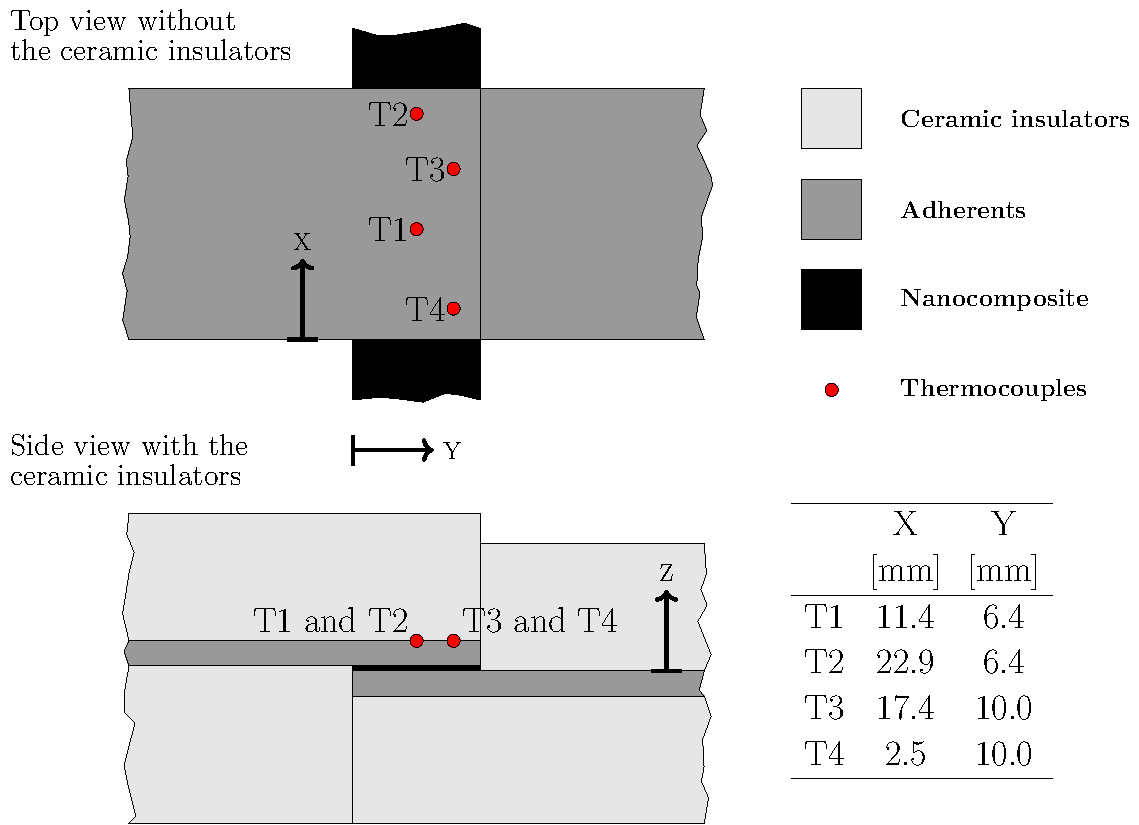
\includegraphics[scale=0.75]{2_Fig3}
	\caption{Location of thermocouples during welding experiments}
	\label{fig:2_Fig3}
\end{figure} 

\FloatBarrier
%%%%%%%%%%%%%%%%%%%%%%%%%%%%%%%%%%%%%%%%%%%%%%%%%%%%%%%%%%%%%%%%%
\section{Results and discussion}
%%%%%%%%%%%%%%%%%%%%%%%%%%%%%%%%%%%%%%%%%%%%%%%%%%%%%%%%%%%%%%%%%

%%%%%%%%%%%%%%%%%%%%%%%%%%%%%%%%%%%%%%%%%%%%%%%%%%%%%%%%%%%%%%
\subsection{Material characterization}
%%%%%%%%%%%%%%%%%%%%%%%%%%%%%%%%%%%%%%%%%%%%%%%%%%%%%%%%%%%%%%

The $C_p$ obtained by MDSC are presented at Table \ref{tab:table1}. 
The thermal conductivity as a function of temperature for CF/PEEK, the PEI/MWCNT nanocomposite and the alumina silicate are reported in Table \ref{tab:table2}. 
The asperities roughness $\sigma_{asp}$ and asperities average slopes $m_{asp}$ were measured respectively at \mbox{0.26\,$\mu$m} and 0.15. 
The microhardness was set at \mbox{0.1\,GPa} in the model. 

\begin{table}[ht]
	\centering
	\begin{tabular}{@{}cccc@{}}
		\toprule
		   Temperature    &           CF/PEEK            &          PEI/MWCNT           &       Alumina Silicate       \\
		{[}$^{\circ}$C{]} & {[}J\,kg$^{-1}$\,K$^{-1}${]} & {[}J\,kg$^{-1}$\,K$^{-1}${]} & {[}J\,kg$^{-1}$\,K$^{-1}${]} \\ \midrule
		       40         &             926              &             1059             &                              \\
		       97         &                              &                              &             975              \\
		       139        &             1265             &                              &                              \\
		       159        &             1359             &                              &                              \\
		       207        &                              &             1561             &                              \\
		       227        &                              &             1765             &                              \\
		       310        &             1809             &                              &                              \\
		       343        &             2400             &                              &                              \\
		       360        &             1792             &                              &                              \\
		       399        &             1790             &             1955             &                              \\ \bottomrule
	\end{tabular}
	\caption{Results for Specific heat measurements}
	\label{tab:table1}
\end{table}

\begin{table}[ht]
	\centering
	\begin{tabular}{@{}ccccc@{}}
		\toprule
		   Temperature    &           CF/PEEK           &           CF/PEEK           &          PEI/MWCNT          &      Alumina Silicate       \\
		                  &          Parallel           &        Perpendicular        &                             &                             \\
		{[}$^{\circ}$C{]} & {[}W\,m$^{-1}$\,K$^{-1}${]} & {[}W\,m$^{-1}$\,K$^{-1}${]} & {[}W\,m$^{-1}$\,K$^{-1}${]} & {[}W\,m$^{-1}$\,K$^{-1}${]} \\ \midrule
		       20         &            2.25             &            0.55             &            0.41             &                             \\
		       40         &                             &                             &            0.30             &             5.7             \\
		       60         &                             &                             &            0.43             &                             \\
		       110        &                             &                             &            0.46             &                             \\
		       150        &                             &                             &            0.48             &                             \\
		       200        &            3.02             &            0.73             &                             &                             \\ \bottomrule
	\end{tabular}
	\caption{Results for thermal conductivity measurement}
	\label{tab:table2}
\end{table}

\FloatBarrier
%%%%%%%%%%%%%%%%%%%%%%%%%%%%%%%%%%%%%%%%%%%%%%%%%%%%%%%%%%%%%%
\subsection{Modelling results}
%%%%%%%%%%%%%%%%%%%%%%%%%%%%%%%%%%%%%%%%%%%%%%%%%%%%%%%%%%%%%%

The model was first validated with experimental data. 
Four resistance welding experiments under different conditions served as references. 
The same welding conditions were reproduced by the model and the resulting validation curves are presented in \mbox{Fig. \ref{fig:2_Fig4}}. 
Initial modelling efforts neglected the electrical contact resistance between the electrodes and the nanocomposite and did not fit the observations. 
Upon further inspection, the contact electrical resistance was measured by subtracting the theoretical nanocomposite’s HE electrical resistance to the total resistance of the welding setup between both electrodes measured with a handheld multimeter. 
The electrical contact resistance accounts for approximately 50\% of the total electrical resistance of the setup. 
Reducing the power by 45\% provided a good agreement with the experiments allowing for the model to explore the general behaviour of the welding process. 

\begin{figure}[ht]
	\center
	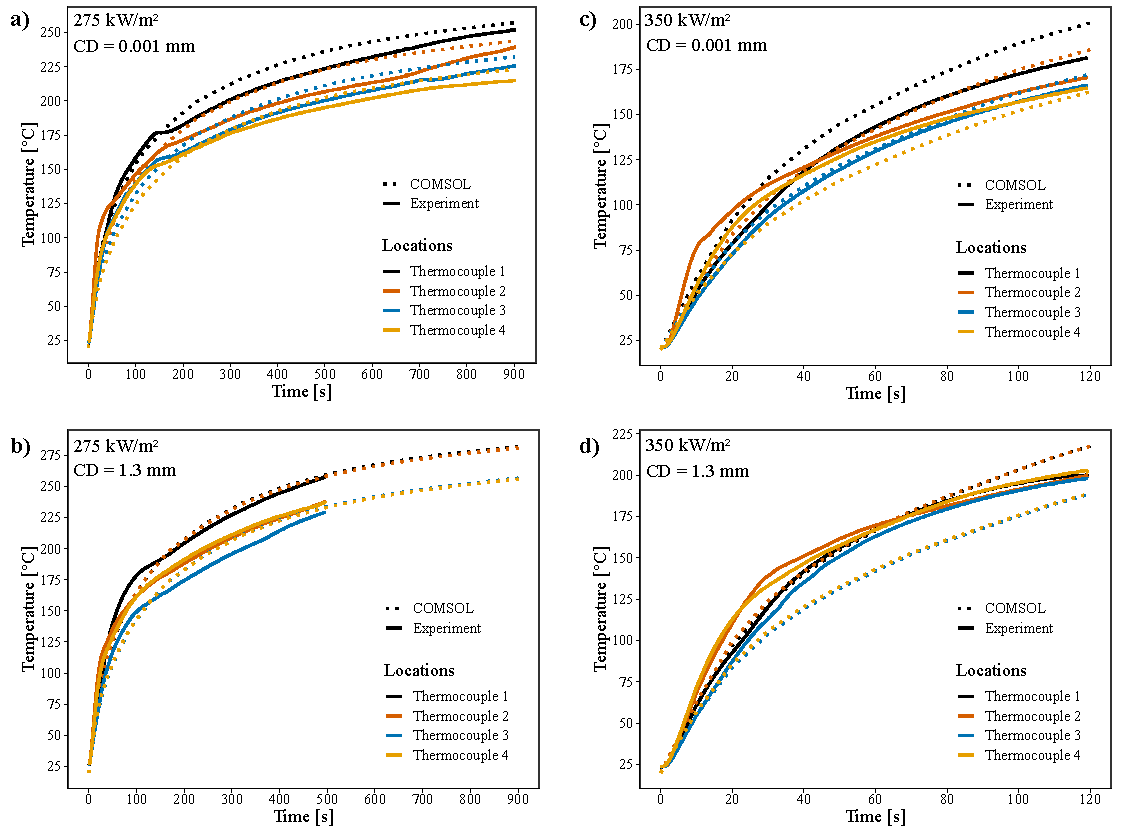
\includegraphics[width=0.95\textwidth]{2_Fig4}
	\caption{Validation curves for the model under various welding conditions with solid line representing experimental results, dotted lines for COMSOL results and colours assigned to each thermocouple locations \cite{Brassard2019b}}
	\label{fig:2_Fig4}
\end{figure} 

\FloatBarrier
As it was not possible to monitor the temperature directly at the weld interface without disturbing the thermal profile and affecting the results, the model offers us insight that could not be obtained from experiments. 
The temperature distribution along the length of the weld (\textit{x-axis}) varies based on the clamping distance and power density, as previously reported \cite{Talbot2013} (\mbox{Fig. \ref{fig:2_Fig5}}). 
It can be controlled with a variation of the clamping distance but the profile across the width of the weld (\textit{y-axis}) is mostly unaffected by the clamping distance. 
A cold edge (at y = \mbox{0\,mm} in \mbox{Fig. \ref{fig:2_Fig5}}) is always present at the top surface of the nanocomposite on the side where the adherent exits the weld due edge effects caused by the high axial thermal conductivity of the carbon fibres in the UD TPC adherents. 
On the bottom surface of the nanocomposite, the cold edge is located on the mirror side of the weld (at y = \mbox{12.7\,mm}) due to the adherent leaving the weld on the other side (details in bottom sections of \mbox{Fig. \ref{fig:2_Fig2}} and \mbox{Fig. \ref{fig:2_Fig3}}). 

\begin{figure}[ht]
	\center
	\includegraphics[width=\textwidth]{2_Fig5}
	\caption{Temperature distributions after 900 and 120 seconds for respective power densities of 275 and 350 kW/m2 at the interface on top of the nanocomposite HE with clamping distances of 0.001, 1.3 and 2.0 mm \cite{Brassard2019b}}
	\label{fig:2_Fig5}
\end{figure} 

\FloatBarrier
Simulations were performed to observe the temperature uniformity along the length of the weld (\textit{x-axis}) to optimize the clamping distance and to evaluate the sensitivity of this parameter. 
The optimal clamping distance is the distance which minimizes the temperature difference between the centre of the weld and the maximum temperature at the edges. 
Polymer degradation at the edge begins when the clamping distance is too large. 
The clamping distances for both conditions vary almost linearly as a function of the power density over the experimental domain (\mbox{Fig. \ref{fig:2_Fig6}}). 
Additionally, an almost constant difference of \mbox{0.4\,mm} exists between the optimal clamping distance and the length causing thermal degradation at the edge. 
Thus, the dimensional tolerance for the location of the electrodes during the resistance welding with a nanocomposite HE process can be on the order of a few tenths of millimetres. 

\begin{figure}[ht]
	\center
	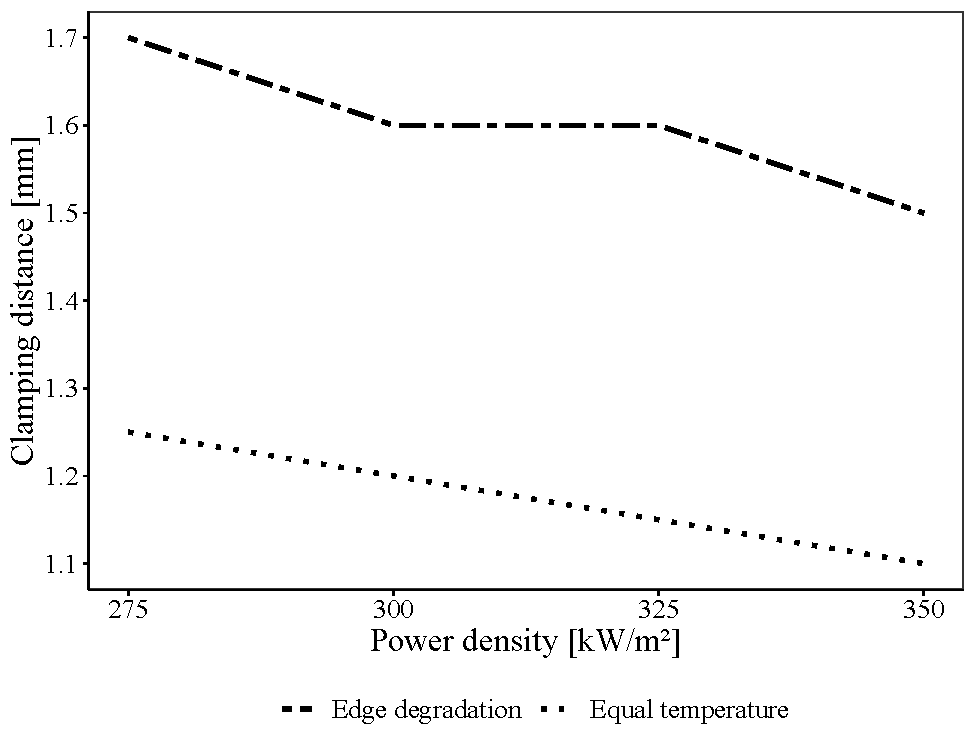
\includegraphics[scale=0.75]{2_Fig6}
	\caption{Sensitivity analysis for the clamping distance showing the clamping distances resulting in optimal temperature distribution and the beginning of edge degradation as a function of power density \cite{Brassard2019b}}
	\label{fig:2_Fig6}
\end{figure} 

It is now possible to expand the scope of the analysis. 
The resulting process window (\mbox{Fig. \ref{fig:2_Fig7}}) presents the time required for the hottest point at the interface to reach \mbox{370\,$^{\circ}$C}, \mbox{400\,$^{\circ}$C} and \mbox{440\,$^{\circ}$C}, \mbox{10\,$^{\circ}$C} below the degradation temperature of PEI \cite{Carroccio2000}. 
The temperature of the lower bound and the average temperature within the weld at that moment (approximately \mbox{390\,$^{\circ}$C}) are higher than the reported temperatures required to obtain reptation times compatible with the resistance welding process for PEI/PEEK interfaces \cite{Bastien1991}. 
On the other hand, the addition of a large fraction of MWCNT is limiting polymer chain mobility at lower temperatures \cite{Mu2009,Kabanemi2010} and a higher temperature or more time is required to achieve similar diffusion of the chains. 
Additional welding experiments were conducted based on the suggested processing window and previous results to validate the model’s results. 
The average single lap shear strength for all welded joints are presented in \mbox{Fig. \ref{fig:2_Fig7}}.  

\begin{figure}[ht]
	\center
	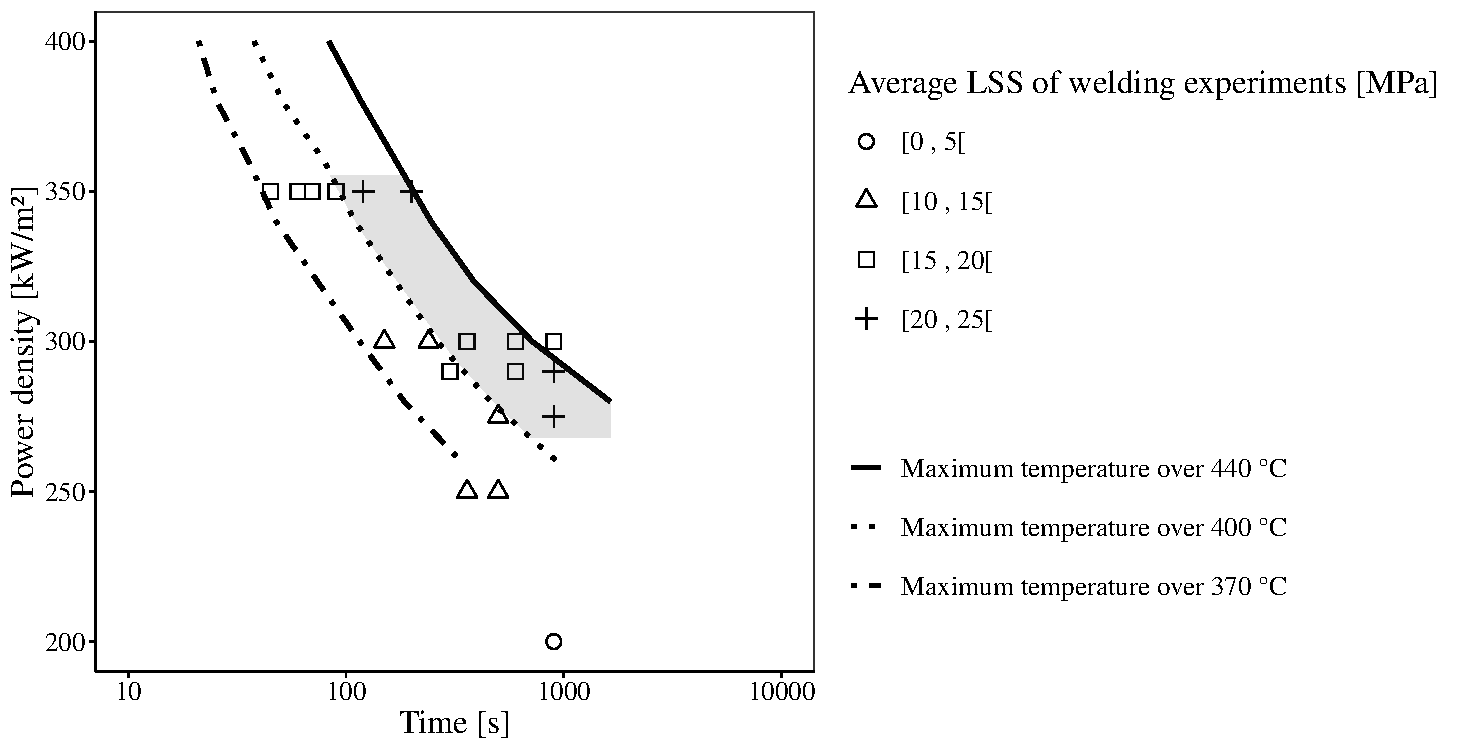
\includegraphics[width=\textwidth]{2_Fig7}
	\caption{Process window (grayed zone) based on the simulation results with optimal clamping distance, the lines represent the time to reach a local maximum temperatures of 370\,$^{\circ}$C, 400\,$^{\circ}$C and 440\,$^{\circ}$C on the top surface of the nanocomposite in the model while the markers presents the single lap shear results from all the welding experiments \cite{Brassard2019b}}
	\label{fig:2_Fig7}
\end{figure} 

\FloatBarrier
%%%%%%%%%%%%%%%%%%%%%%%%%%%%%%%%%%%%%%%%%%%%%%%%%%%%%%%%%%%%%%
\subsection{Welding experiments}
%%%%%%%%%%%%%%%%%%%%%%%%%%%%%%%%%%%%%%%%%%%%%%%%%%%%%%%%%%%%%%

Current leakage in the composite adherents can be a problem for resistance welding of carbon fibre laminates at high power and it currently limits resistance welding with a nanocomposite HE to unidirectional adherents. 
The model pointed toward the possibility to produce welds at lower power and longer times to reduce the voltage difference along the length of the nanocomposite HE to minimize the risk of current leakage. 
Successful welding tests were performed with power densities as low as \mbox{250\,kW\,m$^{-2}$} (resulting LSS $\sim$ \mbox{14\,MPa}). 
These additional tests, along with previous results are included in \mbox{Fig. \ref{fig:2_Fig7}} and in \mbox{Table \ref{tab:table3} and \ref{tab:table4}}. 
The highest average LSS (\mbox{24.9\,MPa}) was obtained at a power density of \mbox{350\,kW\,m$^{-2}$}, a clamping distance of \mbox{1.3\,mm}, a pressure of \mbox{1\,MPa} on the weld and a welding time of \mbox{120\,s}. 
This LSS corresponds to a 28\% improvement relative to previously published results, thanks to a better processing window predicted by the finite element model, with LSS ranging from 14.1 to \mbox{35.2\,MPa}. 
LSS results of joints welded using non-optimal sets of welding parameters are also presented in Table \ref{tab:table3} and \ref{tab:table4} \cite{Brassard2019b}. 
A welding experiment at \mbox{200\,kW\,m$^{-2}$} during \mbox{900\,s} did not result in a successful weld.  

\begin{table}[htb]
	\centering
	\resizebox{0.98\textwidth}{!}{
		\begin{tabular}{@{}lll L{1.6cm} l C{1.1cm} C{1.1cm} C{1.1cm} C{1.1cm} C{1.1cm} C{1.1cm} C{1.1cm} @{}}
		\toprule
		Power              & Clamping & Pressure  & Values            &       &                                                         \multicolumn{7}{c}{Time}                                                          \\
		density            & distance &           &                   &       &                                                        \multicolumn{7}{c}{{[}s{]}}                                                        \\
		{[}kW\,m$^{-2}${]} & {[}mm{]} & {[}MPa{]} &                   &       & 45                & 60                & 70                & 90                & 120               & 150               & 200               \\ midrule
		300                & 1.2      & 1.0       & LSS \mbox{± S.D.} & [MPa] &                   &                   &                   &                   &                   & 14.9 \mbox{± 5.6} &                   \\
		                   &          &           & Samples           &       &                   &                   &                   &                   &                   & 3                 &                   \\
		350                & 0        & 1.0       & LSS \mbox{± S.D.} & [MPa] &                   &                   &                   &                   & 15.2 \mbox{± 1.7} &                   &                   \\
		                   &          &           & Samples           &       &                   &                   &                   &                   & 4                 &                   &                   \\
		                   & 1.0      & 1.0       & LSS \mbox{± S.D.} & [MPa] &                   &                   &                   &                   & 13.0 \mbox{± 4.4} &                   &                   \\
		                   &          &           & Samples           &       &                   &                   &                   &                   & 3                 &                   &                   \\
		                   & 1.1      & 1.0       & LSS \mbox{± S.D.} & [MPa] & 17.4 \mbox{± 3.6} &                   &                   &                   &                   &                   & 21.0 \mbox{± 5.6} \\
		                   &          &           & Samples           &       & 3                 &                   &                   &                   &                   &                   & 3                 \\
		                   & 1.3      & 1.0       & LSS \mbox{± S.D.} & [MPa] &                   &                   &                   &                   & 24.9 \mbox{± 9.7} &                   &                   \\
		                   &          &           & Samples           &       &                   &                   &                   &                   & 4                 &                   &                   \\
		                   & 1.5      & 1.0       & LSS \mbox{± S.D.} & [MPa] &                   & 16.4 \mbox{± 7.8} & 18.6 \mbox{± 2.0} & 15.5 \mbox{± 3.8} & 19.6 \mbox{± 3.5} &                   &                   \\
		                   &          &           & Samples           &       &                   & 3                 & 3                 & 3                 & 3                 &                   &                   \\ \bottomrule
		\end{tabular}}
	\caption{LSS tests results}
	\label{tab:table3}
\end{table}

\begin{table}[htb]
	\centering
	\resizebox{0.98\textwidth}{!}{
		\begin{tabular}{@{}lll L{1.6cm} l C{1.1cm} C{1.1cm} C{1.1cm} C{1.1cm} C{1.1cm} C{1.1cm}@{}}
			\toprule
			Power              & Clamping & Pressure  & Values            &           &                                             \multicolumn{6}{c}{Time}                                               \\
			density            & distance &           &                   &           &                                             \multicolumn{6}{c}{{[}s{]}}                                              \\
			{[}kW\,m$^{-2}${]} & {[}mm{]} & {[}MPa{]} &                   &           & 240               & 300               & 360               & 500              & 600               & 900               \\ \midrule
			200                & 0        & 1.0       & LSS \mbox{± S.D.} & {[}MPa{]} &                   &                   &                   &                  &                   & 3.1 \mbox{± NA}   \\
			                   &          &           & Samples           &           &                   &                   &                   &                  &                   & 1                 \\
			250                & 0        & 1.0       & LSS \mbox{± S.D.} & {[}MPa{]} & 13.2 \mbox{± NA}  &                   & 14.1 \mbox{± NA}  &                  &                   &                   \\
			                   &          &           & Samples           &           & 1                 &                   & 1                 &                  &                   &                   \\
			275                & 0        & 1.0       & LSS \mbox{± S.D.} & {[}MPa{]} &                   &                   &                   &                  &                   & 20.0 \mbox{± 2.7} \\
			                   &          &           & Samples           &           &                   &                   &                   &                  &                   & 4                 \\
			                   & 1.3      & 1.0       & LSS \mbox{± S.D.} & {[}MPa{]} &                   &                   &                   & 24.3 \mbox{± NA} &                   &                   \\
			                   &          &           & Samples           &           &                   &                   &                   & 1                &                   &                   \\
			290                & 0        & 1.0       & LSS \mbox{± S.D.} & {[}MPa{]} &                   &                   &                   &                  &                   & 17.8 \mbox{± 2.2} \\
			                   &          &           & Samples           &           &                   &                   &                   &                  &                   & 4                 \\
			                   &          & 1.4       & LSS \mbox{± S.D.} & {[}MPa{]} &                   &                   &                   &                  &                   & 21.4 \mbox{± 2.7} \\
			                   &          &           & Samples           &           &                   &                   &                   &                  &                   & 2                 \\
			                   & 1.2      & 1.0       & LSS \mbox{± S.D.} & {[}MPa{]} &                   & 18.9 \mbox{± 7.0} &                   &                  & 17.7 \mbox{± 4.3} &                   \\
			                   &          &           & Samples           &           &                   & 3                 &                   &                  & 3                 &                   \\
			300                & 0        & 1.0       & LSS \mbox{± S.D.} & {[}MPa{]} & 13.8 \mbox{± 3.8} &                   & 17.7 \mbox{± 1.1} &                  &                   & 16.5 \mbox{± 0.7} \\
			                   &          &           & Samples           &           & 3                 &                   & 3                 &                  &                   & 3                 \\
			                   & 1.2      & 1.0       & LSS \mbox{± S.D.} & {[}MPa{]} &                   &                   &                   &                  & 19.4 \mbox{± 3.0} &                   \\
			                   &          &           & Samples           &           &                   &                   &                   &                  & 3                 &                   \\ \bottomrule
		\end{tabular}}
	\caption{LSS tests results (continued)}
	\label{tab:table4}
\end{table}

\FloatBarrier
%%%%%%%%%%%%%%%%%%%%%%%%%%%%%%%%%%%%%%%%%%%%%%%%%%%%%%%%%%%%%%
\subsection{Nanocomposite tensile strength}
%%%%%%%%%%%%%%%%%%%%%%%%%%%%%%%%%%%%%%%%%%%%%%%%%%%%%%%%%%%%%%

Due to the high loading of MWCNTs in the nanocomposite, it is expected that its ductility and tensile strength are impacted. 
Average tensile strength of 72.2 $\pm$ \mbox{19.4\,MPa} and elongation at break of 5.2 $\pm$ 1.7\% were obtained from tensile tests on nanocomposite samples. 
During these tests, all samples had brittle failure mode without a ductile plateau. 
This can be contrasted to virgin properties of ULTEM 1010 (tensile strength of 110 MPa and 60\% elongation) to show that the mechanical behaviour of the nanocomposite is severely affected by the 10\% wt. loading of MWCNTs, which was also noticeable during the handling of the HE. 
The variability in the performances of the nanocomposite is in line with the variability observed in the LSS tests. 

%%%%%%%%%%%%%%%%%%%%%%%%%%%%%%%%%%%%%%%%%%%%%%%%%%%%%%%%%%%%%%
\subsection{Fractography}
%%%%%%%%%%%%%%%%%%%%%%%%%%%%%%%%%%%%%%%%%%%%%%%%%%%%%%%%%%%%%%

Direct imaging of the fractured surfaces (\mbox{Fig. \ref{fig:2_Fig8}}) provided some insight on the failure modes of the welded joints. 
First, signs of unstable crack propagation due to the brittleness of the nanocomposite are clearly visible. 
Evenly spaced cracks in the matrix residues are visible on one face (\mbox{Fig. \ref{fig:2_Fig8}}a) and evenly spaced ridges are visible in the mirror matching face (\mbox{Fig. \ref{fig:2_Fig8}}b). 
A close look at those ridges (\mbox{Fig. \ref{fig:2_Fig8}}c) shows polymer well bonded to the composite substrate. 
Additionally, broken fibres can be seen embedded on top of nanocomposite residues still attached to opposing faces (\mbox{Fig. \ref{fig:2_Fig8}}d). 
Both of these observations are signs that the bonding between the nanocomposite and the composite adherents is not the weakest link. 
Signs of thermal degradation could be observed in \mbox{Fig. \ref{fig:2_Fig8}}e serving as an example of porosities left by vaporized polymer. 
Carbon fibres with no polymer attached to them or degraded polymer residues can be seen at other locations. 
Finally, when thermal degradation and unstable cracks combine in the same zone, a different failure mode can be observed where cracks form between adjacent porosities and through the nanocomposite (\mbox{Fig. \ref{fig:2_Fig8}}f).

\begin{figure}[htb]
	\center
	\includegraphics[width=0.98\textwidth]{2_Fig8}
	\caption{SEM fractography of welded specimens showing a) unstable crack propagation causing evenly spaced cracks in the nanocomposite b) and c) ridges left on the opposing surface when cracks forms d) fibre adherence to the nanocomfig:Figposite HE e) signs of localized thermal degradation f) unstable crack propagation combined with thermal degradation \cite{Brassard2019b}}
	\label{fig:2_Fig8}
\end{figure} 

The SEM observations, reduced tensile strength and low elongation at break of the nanocomposite combine to infer that the current limiting factor for resistance welding of thermoplastic composites with a nanocomposite HE is the nature of the nanocomposite itself. 
In traditional resistance welding, a compliant resin rich layer is present between the adherents and can dissipate energy through plastic deformation. 
With the current brittle nanocomposite, as soon as cracking occurs, cracks will propagate in an unstable fashion through the interface. 
Improvements to the process could come either by combining the brittle nanocomposite with an underlying compliant layer of material to produce a flexible joint or by modifying the composition of the nanocomposite to increase its ductility while maintaining its electrical conductivity. 

\FloatBarrier
%%%%%%%%%%%%%%%%%%%%%%%%%%%%%%%%%%%%%%%%%%%%%%%%%%%%%%%%%%%%%%%%%
\section{Conclusion}
%%%%%%%%%%%%%%%%%%%%%%%%%%%%%%%%%%%%%%%%%%%%%%%%%%%%%%%%%%%%%%%%%

This work presented the development of a finite element model for the resistance welding of thermoplastic composites, using a nanocomposite heating element. 
The model allowed to establish a processing window leading to an improvement of up to 28\% in the LSS of welded joints. 
Furthermore, the model and new experiments presented here increased our knowledge of the phenomena at play when welding using these newly developed HE. 
The model hinted at the possibility to produce welds at lower power densities and this was validated experimentally. 
Finally, mechanical testing and fractography analysis of the nanocomposite HE highlighted its brittle nature which is currently the limiting factor in the mechanical strength of the welded joints. 
Future work will aim at producing a conductive nanocomposite with a higher ductility than the current solution or to bond the nanocomposite to a compliant intermediary layer. 

%%%%%%%%%%%%%%%%%%%%%%%%%%%%%%%%%%%%%%%%%%%%%%%%%%%%%%%%%%%%%%%%%
\section{Acknowledgements}
%%%%%%%%%%%%%%%%%%%%%%%%%%%%%%%%%%%%%%%%%%%%%%%%%%%%%%%%%%%%%%%%%

This work was supported by ArianeGroup and CREPEC. 
The authors would also like to thank Vincent Rohart for his time and help for the SEM imaging and Prof. Philippe Pasquier for the thermal conductivity measurements. 